\documentclass{article}
% To modify the size of the page:
\usepackage[dvips,a0paper,landscape,centering,left=5cm,right=5cm,top=5cm, bottom=5cm]{geometry}
\usepackage[english, serbian c]{babel}
\usepackage{multicol}
\usepackage[utf8]{inputenc}
\usepackage{color,xcolor}
\usepackage{float}
\usepackage{amsmath, amsthm, amsfonts}
\usepackage{graphicx}           % Include figure files.
\usepackage{anyfontsize}
\usepackage{setspace}
\usepackage{lipsum}
% Colors
% -------
\usepackage[immediate]{silence}
\WarningFilter[temp]{latex}{Command} % silence the warning
\definecolor{azulcielo}{RGB}{227,243,248}

\newcommand\Mark[1]{\textsuperscript#1}
\pagestyle{empty}

\def\to{\rightarrow}
\usepackage{geometry}
\usepackage{layout}
\usepackage{url}
\usepackage[pdftex, pdfborderstyle={/S/U/W 0}]{hyperref}
\usepackage{csquotes}
\usepackage[backend=biber, style=ieee,language=auto]{biblatex}
\addbibresource{bibliography.bib}

\graphicspath{{media/images/}}
\DeclareGraphicsExtensions{.jpeg,.png,.jpg}
\usepackage{sectsty}
\sectionfont{\fontsize{60}{72}\selectfont}

% ===========================================================================

\title{}
\author{}
\date{}

\begin{document}
%\maketitle

\begin{center}
  \begin{minipage}{.16\linewidth}
  \qquad\qquad
    
\includegraphics[width=.7\linewidth]{media/images/grb.png}
    ~\vfill
    ~\vfill
  \end{minipage}
  %&
  \begin{minipage}{.6\linewidth}
    \begin{center}
       \textsf{\textbf{{\fontsize{90}{108}\selectfont Дигиталне урбане мреже и друштвени медији}}}\\\vspace{1cm}
       \textrm{\fontsize{40}{48}\selectfont Тамара Јевтимијевић, 261/2017 \\\vspace{5mm} \textit{Рачунарство и друштво}, \textit{Математички факултет у Београду}\\\vspace{10mm} Email: mi17261@alas.matf.bg.ac.rs}  
    \end{center}
  \end{minipage}
  %&
  \hspace{.03\linewidth}
    \begin{minipage}{.16\linewidth}
  \qquad\qquad
    
\includegraphics[width=.7\linewidth]{media/images/grb.png}
    ~\vfill
    ~\vfill
  \end{minipage}
\end{center}

\vspace{2cm}

% ---------------------------------------------------------------------------
\fontsize{30}{36}\selectfont
\setlength{\columnsep}{1cm}
\begin{multicols}{3}
% ---------------------------------------------------------------------------

\noindent
\fcolorbox{black}{azulcielo}{
  \begin{minipage}[H]{.96\linewidth}
    \begin{center}
      \vspace{1cm}
      \section*{Сажетак}
      Златна грозница данашњег времена се односи на
рударење података за комерцијалну употребу. У циљу зараде и комерцијализације
корпорације, које се баве информационо-комуникационим технологијама, често активно и агресивно нуде услуге на рачун опште популације. Заједно са паметним градом, концепт безбедног града је такође пример где корпорације, које се баве информационо-комуникационим технологијама имају највише утицаја и може се рећи да је рударења података стратегија за обогаћивање тих корпорација. Крајем двадесетог и почетком двадесет првог века ИКТ корпорације су доживеле највећу експанзију. Данас их има све више и све су више утицајне. Технологија је узнапредовала великом брзином и своје гране је пустила свуда. Данас где год да се окренемо дигитализација је око нас. У наставку ће бити више речи о томе како је дигитализација допринела развоју градова, побољшању живота људи у градовима и како су технологије заокупирале читав свет.
      \vspace{1cm}
    \end{center}
  \end{minipage}
  
}
\section*{}

\noindent Како се повећавају урбани изазови, пропагирани урбанизацијом и растом становништва, већина градова се окренула коришћењу различитих модерних технологија. Разлози за прихватање технологија су сазнање да технологије, коришћењем података генерисаних из града у ком се користе, имају потенцијал да пруже дугорочно решење, које утиче на ефикасности и исплативости живота у градовима. \\\\
Са разноликим технологијама, посебно оним, које су удружене са концептом паметног града, повећала се могућност праћења изазова и потреба становништва.

\section*{Друштвене мреже и град}
\noindent Успон друштвених мрежа као што су Facebook, Twitter, WeChat, Tumblr, Instagram, Google+, YouTube, Linkedin, TikTok, Snapchat и WhatsApp такође је променио начин на који људи широм света комуницирају и живе. Чини се да људи више воле и примењују дигиталне интеракције у односу на физичке интеракције. 
Процењује се да преко 3,2 милијарде људи широм света користите друштвене мреже на овај или онај начин, а ови трендови су заслужни за широк продор паметних уређаја као што су мобилни телефони и таблети. Друштвене мреже су имале свој утицај у областима попут управљања, економског раста, безбедности, образовања, здравственог сектора и транспортног сектора и у још многим другим сферама и областима.

\begin{center}
    \vspace{1cm}
    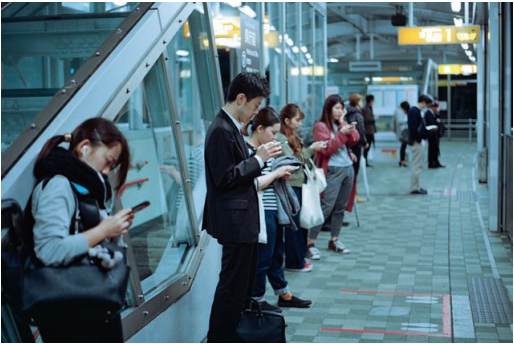
\includegraphics[width=0.9\linewidth]{media/images/drustvene_mreze.png}
\end{center}
% ---------------------------------------------------------------------------
\section*{Урбано брендирање и друштвене мреже}
\noindent Појава дигиталних решења која се фокусирају на градове и урбана подручја је имала бројне позитивне стране као што је могућност брендирања града. Дигитални бренд је дао градовима прилику да дигиталне технологије искористе на економској граници. Након појаве друштвених мрежа, туристички брендови су прихваћени у различитим градовима кроз стратегије прилагођене различитим корисницима на различитим платформама друштвених мрежа. \\
На пример, Амстердам, уметнички град са култним музејима ибогатом историјом, усвојио је израз „I AMSTERDAM“, приказан на знаку који носи ту фразу и налази се испед музеја Rijksmuseum. Знак има велику моћ привлачења туриста у град. Његова популарност је дошла захваљујући Твитер хештегу „#IAmsterdam“, који га је промовисао до те мере да га је приметио велики број људи и да је преко 6000 селфија снимљено испред њега сваког дана и већина њих је подељена путем Твитера. Брендирање је стратегија која је невино усвојена, да би се они, који су у овом случају живели у Аместердаму и у њему радили, али и они који су га само посетили осетили његовим делом. Брендирање је у случају Амстердама имало огроман утицај које је резултовао тиме да је град увек био пренасељен до тачке да је тема туризма постала контрапродуктивна.

\begin{center}
    \vspace{1cm}
    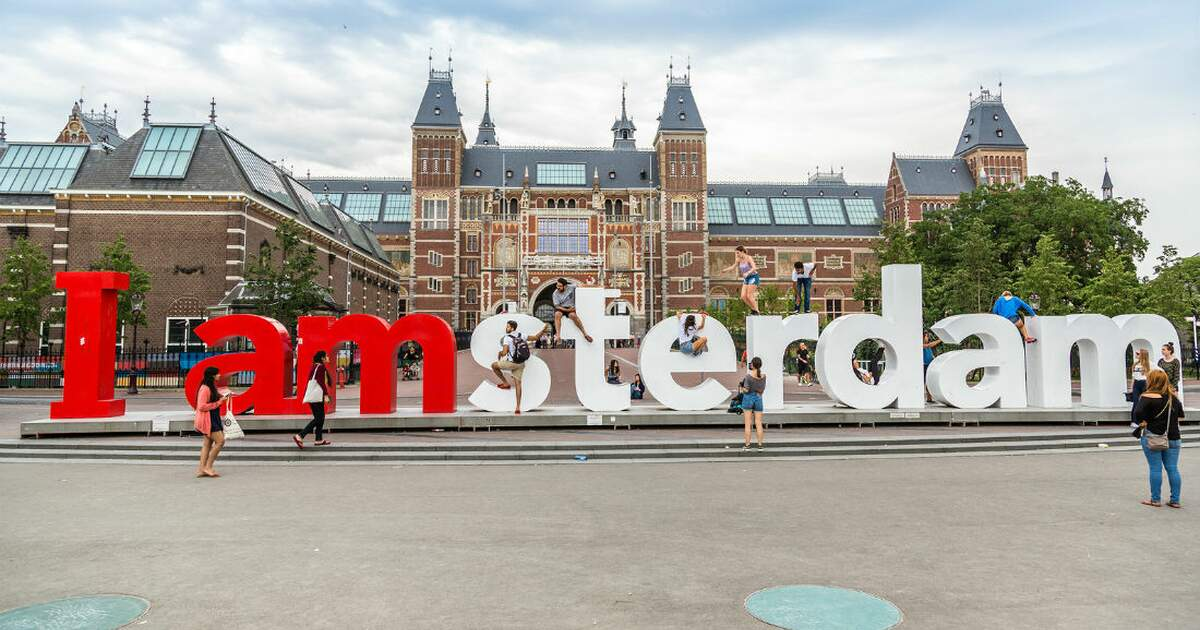
\includegraphics[width=0.9\linewidth]{media/images/rijksmuseum-amsterdam-museum-iamsterdam.jpg}
\end{center}

\section*{Закључак}

\noindent Можемо приметити све већу улогу дигиталних медија у
обликовању градске привреде и политичке сфере. Улога друштвених медија односно мрежа у градовима, посебно у јавним просторима, постају све више наглашени, а види се да политичари све више користе те платформе како би стекли политичку километражу и економску отпорност крозповећање активности у вези са туризмом коришћењем нових, технолошки прилагођених техника брендирања и маркетинга.
% ---------------------------------------------------------------------------
%

\end{multicols}

\end{document}
